\scanpage{411}
\mspage{208}

and unless I am mistaken, it has become obvious
that this functor is an \uline{equivalence of
categories} (and as a consequence, there
\margin{\unsure{for the} \uline{\unsure{isomorphisms}}}
is the functor in the opposite direction :
drill holes at ``points'' invariant
under $\Gamma_{\unsure{a|0}}$ (or at arbitrary points,
at the cost of passing to a smaller $\Gamma'$).

But I realize that
\deleted{\illegible{1}} this is not at all obvious -- I am going
to try to elucidate the situation axiomatically.
We have fixed a genus $g$,
we suppose given, for varying $\nu$
(such that $(g,\nu)$ anabelian) closed
subgroups $N_{g,\nu}\subset\widehat{\widehat{\mathcal T}}_{g,\nu}$,
normalizing $\widehat{\mathcal T}_{g,\nu}$, and satisfying the
essential condition that the $\psi_i:\widehat{\widehat{\mathcal T}}_{g,\nu}\longrightarrow\widehat{\widehat{\unsure{\mathcal G|\mathcal S}}}_{g,\nu-1}$
induce
\[
M_{g,\nu}\xrightarrow{\sim}M_{g,\nu-1}
\]
Which makes it possible to define the notion
of arithmetization of a profinite $\pi$ of
anabelian type $(g,\nu)$, and the theory of

\scanpage{412}

plugging an arbitrary number of holes, and
of drilling just 1 hole, in the
category of groups of type $g,\nu$,
arithmetized.

We suppose on the other hand \unsure{given|given} a
full subcategory of the category of profinite
\margin{\unsure{we suppose it} : stable under taking open subgroups.}
groups (which could reduce to the
open subgroups of $\mathbb{\Gamma}_g$, common
value of the $\mathbb{\Gamma}_{g,\nu}$ or of open subgroups
of the group $\mathbb{\Gamma}_a$, $a$ an
arithmetization), and \deleted{some} \inserted{a notion of }outer operations
\inserted{``admissible''} of such $\Gamma$ on the
arithmetized $\pi$. We suppose

\textcircled{1} If $\Gamma$ operates admissibly on $\pi$, every
open subgroup too (\deleted{\unsure{and}} and conversely ?)

\textcircled{2} If moreover $\Gamma$ leaves invariant a subset $I'$
of $I=I(\pi)$, then by ``plugging $I'$'',
the operation of $\Gamma$ on $\pi'$ is admissible.

\margin{It suffices to \unsure{postulate it|prove it} for $\operatorname{card} I'=1$, i.e. plugging \unsure{a|a single} hole -- \unsure{at least if we know that the admissibility condition depends only on the action of the kernels of the groups}.}

\deleted{\illegible{1}}
\deleted{\unsure{We propose to define a notion of admissible action} \illegible{2}}
\inserted{When we have an \inserted{\uline{actual}} action, \unsure{(not outer)|(non-outer)}}
of $\Gamma$ on a $(\pi,a)$, then the functor
\unsure{of} ``\deleted{plugging}\inserted{drilling} holes'' gives an outer
action on a $(\pi^0,a^0)$ of type $g,\nu+1$,
and we say that the starting action is

\scanpage{413}
\mspage{209}

admissible, if the \uline{outer} action deduced is.

We thus find an \uline{equivalence} between
the category of \deleted{\unsure{categories}} systems $(\pi,a,\Gamma,\psi,i)$
of a $(\pi,a)$ of type $(g,\nu+1)$, with an
admissible \inserted{\uline{outer}} operation $\psi$ of a $\Gamma$ on it, and
an $i\in I(\pi)$ stable under $\Gamma$, with the category
of $(\pi',a',\Gamma,\psi')$ of $(\pi',a')$ of type
$(g,\nu)$, with a \uline{genuine} admissible action $\psi'$
of $\Gamma$ on it.

\deleted{\unsure{We must} \illegible{3}}
\inserted{Condition (1) ensures that}
\deleted{\textcircled{3} \unsure{If a genuine action}}
\inserted{if $\Gamma$ operates \deleted{\uline{\unsure{genuinely}}} \deleted{\unsure{admissible|admissibly}} actually, in a way}
admissible, then the outer action deduced
is admissible (but the converse will
not be true -- there will be ``pathological''
liftings of a given admissible \unsure{categorical|outer} action\ldots). We suppose moreover

\margin{\figure{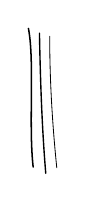
\begin{tikzpicture}[x=1cm,y=1cm,line cap=round,baseline=(current bounding box.center)]
\draw[line width=0.55pt] (0.04,1.80) .. controls (0.12,1.38) and (0.04,0.57) .. (0.10,0.04);
\draw[line width=0.50pt] (0.18,1.74) .. controls (0.19,1.20) and (0.21,0.55) .. (0.26,-0.04);
\draw[line width=0.30pt] (0.31,1.70) .. controls (0.31,1.09) and (0.35,0.52) .. (0.40,0.03);
\end{tikzpicture}}}
\textcircled{3} If $\Gamma$ operates \inserted{actually} in an admissible way on
$\pi$, then $\pi^\Gamma=(1)$.

\deleted{Let \unsure{Then}}
This implies that the category of
$\Gamma$-Points of $\pi$, or if you like of sections
of $B_{\pi,\Gamma}\,(\unsure{\simeq}B_u)$ over $B_\Gamma$, is \uline{rigid}.

\scanpage{414}

But \deleted{\unsure{let us call|let us suppose}} let us consider the inductive limit category of the \deleted{\illegible{1}} categories of sections of $B_{\pi,\Gamma}\simeq B_u$ over $B_{\Gamma'}$ ($\Gamma'$ an open subgroup), it is discrete and corresponds to the set
\[
\mathrm{Pt}_{\mathrm{ad}}(B_{\pi,\Gamma^{\natural}})\simeq
\underset{\substack{\Gamma'\ \mathrm{ouvert}\\\mathrm{de}\ \Gamma}}{\varinjlim}
\mathrm{Pt}_{\mathrm{ad}}(B_{\pi,\Gamma'}).
\]

\margin{\uline{N.B.} The groupoid with strict operators $\uline{\mathrm{Pt}}(B_{\pi,\Gamma})$ depends \unsure{functorially} on $(\pi,\Gamma)$, \illegible{1} for outer morphisms \deleted{\unsure{in}} \unsure{more} \illegible{3} of $\Gamma$, if \deleted{\illegible{4}}.}

\deleted{\textcircled{4} \unsure{For} \illegible{2} $\mathrm{Pt}(B_{\pi,\Gamma})$ \illegible{1}. On the other hand, $\pi$ can be defined by a groupoid.}
If $\mathrm{Pt}(B_{\pi,\Gamma})\ne\varnothing$, then (from the mere fact that $\pi^{\Gamma'}=(1)$ for $\forall$ open subgroup of $\unsure{\Gamma'|\Gamma}$) \inserted{the categorical group} $\pi$ can be described \unsure{canonically|commutatively} by a groupoid \inserted{profinite $\uline{\mathrm{Pt}}(B_{\pi,\Gamma^{\natural}})$} having $\mathrm{Pt}(B_{\pi,\Gamma})$ as object set, \deleted{\unsure{and|then}} \inserted{\unsure{linked|linked} by the categorical group $\pi$, on} which $\Gamma$ operates in the strict sense, with the stabilizer \inserted{$\Gamma_P$} of $\forall$ point being open. and $\Gamma_P\to\mathrm{Aut}(P)$ $(\simeq\pi\ \text{mod \unsure{inner automorphisms}})$

\deleted{More precisely, \unsure{independently of} the preceding axiomatics, we can describe the systems \unsure{formed} of a profinite group \inserted{categorical $\pi$}, and of an \inserted{outer} operation \unsure{of a profinite group} $\Gamma$ on it, \unsure{satisfying}}

being continuous. We have here \unsure{if} to $\forall\ P\in\mathrm{Pt}(B_{\pi,\Gamma})$ we associate the isomorphism class of \deleted{\unsure{groups of liftings}}

\scanpage{415}
\mspage{210}

\deleted{\unsure{groups}} of sections of $B_{\pi,\Gamma}$ over $B_\Gamma$, we find a bijection -- which characterizes the \inserted{$\Gamma$-}groupoid in question up to unique \uline{isomorphism}. We suppose

\textcircled{4} If $\Gamma$ operates admissibly on $(\pi,a)$, then there exists an open subgroup $\Gamma'$ of $\Gamma$ \deleted{can \unsure{operate in a way}} \inserted{whose \inserted{categorical} operation lifts to an} admissible actual operation -- i.e. $\mathrm{Pt}_{\mathrm{ad}}(B_{\Gamma,\pi})\ne\varnothing$.

\deleted{That said, let us consider \deleted{\illegible{1}} the situation of an admissible \inserted{outer} action of $\Gamma$ on $(\pi,a)$ and of an $i\in I(\pi)$ \deleted{stable} fixed under $\Gamma$. We thus have an \uline{actual} action \inserted{\unsure{admissible}} of $\Gamma$ on $(\pi',a')$, \deleted{and moreover we have} \inserted{thus an outer action,} plus a Point ``$\Gamma$-rational'', i.e. invariant under $\Gamma$. Let us consider on the other hand an admissible \unsure{lifting} $\Gamma\longrightarrow M(\pi,a)$, and \illegible{2}}

Let us note that in the situation envisaged, of plugging a hole $i\in I(\pi)$ of a $\pi$, in addition to the homomorphism
\[
\widehat{\widehat{\mathcal T}}(\pi)_i
\xrightarrow{\psi_i}
\widehat{\widehat{\unsure{\mathcal G|\mathcal S}}}(\pi'_i)
\]
associated, giving by composition
\[
\widehat{\widehat{\mathcal T}}(\pi)_i
\xrightarrow{\psi'_i}
\widehat{\widehat{\mathcal T}}(\pi'_i)
\]